\begin{frame}[c]{Batch normalization}
    Initially proposed by \textcite{batchnorm-ioffe15}.
    \bemph{Goal:} Normalize layer input 
    to zero-mean and unit variance (with respect to the current mini-batch).
  
    \begin{algorithm}[H]
      \caption{Batch normalization transform $\eta_{\gamma, \beta}$}
      \textbf{Input:} mini batch $\mathcal{B} = \{x_1, x_2, \dots, x_{n_\mathcal{B}}\} \subset \R^n$ 
      and $x_k \in \mathcal{B}$ \\
      \textbf{Output:} $\eta_{\gamma, \beta}(x_k) \in \R^n$
      %\setstretch{1.5}
      \begin{algorithmic}
        \If{training\_mode} \Comment{Update mean and variance if training, otherwise
        keep previous values}
          \State $\displaystyle
          \mu_\mathcal{B} \gets \frac{1}{n_\mathcal{B}} \sum_{i=1}^{n_\mathcal{B}} x_i$
          \State $\displaystyle
          \sigma^2_\mathcal{B} \gets \frac{1}{n_\mathcal{B}} \sum_{i=1}^{n_\mathcal{B}} 
          (x_i - \mu_\mathcal{B})^2$
        \EndIf
        \State \Return 
        $\displaystyle \lb \frac{\gamma_j}{(\sigma^2_\mathcal{B})_j + \epsilon} 
        \lb (x_k)_j - \lb \mu_\mathcal{B} \rb_j \rb + \beta_j \rb_{j=1}^n$
        \Comment{Here, $\gamma, \beta \in \mathbb{R}^{n}$ are learnable parameters.}
      \end{algorithmic}
    \end{algorithm}
\end{frame}

\begin{frame}{Padding}
    \begin{definition}[Constant padding]
        Given the padding values $l,r \in \mathbb{R}^m$, we define constant padding 
        $c_{\text{pad},m}$ as
        \begin{equation*}
        c_{\text{pad},m} : \mathbb{R}^d \to \mathbb{R}^{d+2m},
        \quad c_{\text{pad},m}(x) = c_{\text{pad},m}(x;l,r) := \lb l^T, x^T, r^T \rb^T
        .
        \end{equation*}
    \end{definition}

    \vspace{0.3cm}
    Example:
    $l,r \in \R^3$,
    $x \in \R^6$

    \vspace{0.3cm}
    \centering
    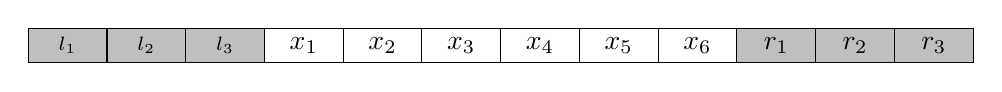
\begin{tikzpicture}
        \node [draw, minimum width=1cm,fill=lightgray] at (0, 0) {\scriptsize$l_1$};
        \node [draw, minimum width=1cm,fill=lightgray] at (1, 0) {\scriptsize$l_2$};
        \node [draw, minimum width=1cm,fill=lightgray] at (2, 0) {\scriptsize$l_3$};
        \foreach \i in {1,2,3,4,5,6} {
        \node [draw, minimum width=1cm] at (\i+2, 0) {$x_\i$};
        }
        \node [draw, minimum width=1cm,fill=lightgray] at (9, 0) {$r_1$};
        \node [draw, minimum width=1cm,fill=lightgray] at (10, 0) {$r_2$};
        \node [draw, minimum width=1cm,fill=lightgray] at (11, 0) {$r_3$};
    \end{tikzpicture}
\end{frame}

\begin{frame}{Padding}
    \begin{definition}[Symmetric padding]
        We define symmetric padding as
        \begin{equation*}
        s_{\text{pad},m} : \mathbb{R}^d \to \mathbb{R}^{d+2m},
        \quad s_{\text{pad},m}(x) := (
            \underbrace{x_m, x_{m-1} \dots, x_1}_{m \text{ values}}, \,
            \underbrace{x_1, x_2 \dots, x_d}_{d \text{ values}}, \,
            \underbrace{x_d, x_{d-1} \dots, x_{d-m+1}}_{m \text{ values}}
        )^T
        .
        \end{equation*}
    \end{definition}

    \vspace{0.3cm}
    Example:
    $x \in \R^6$

    \vspace{0.3cm}
    \centering
    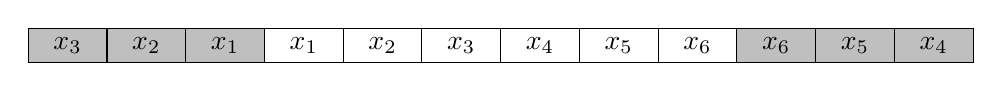
\begin{tikzpicture}
        \node [draw, minimum width=1cm,fill=lightgray] at (0, 0) {$x_3$};
        \node [draw, minimum width=1cm,fill=lightgray] at (1, 0) {$x_2$};
        \node [draw, minimum width=1cm,fill=lightgray] at (2, 0) {$x_1$};
        \foreach \i in {1,2,3,4,5,6} {
        \node [draw, minimum width=1cm] at (\i+2, 0) {$x_\i$};
        }
        \node [draw, minimum width=1cm,fill=lightgray] at (9, 0) {$x_6$};
        \node [draw, minimum width=1cm,fill=lightgray] at (10, 0) {$x_5$};
        \node [draw, minimum width=1cm,fill=lightgray] at (11, 0) {$x_4$};
    \end{tikzpicture}
\end{frame}

\begin{frame}{Semi-linear wave equation}
    One-dimensional semi-linear wave equation with constant speed $c \in \R$, nonlinear term 
    $g : \R \to \R$, domain length $l \in \R$ and domain $\Omega = [-l/2, l/2]$:
    \begin{equation*}
        \frac{\partial^2}{\partial t^2} u(t,x) = 
        c^2 \frac{\partial^2}{\partial x^2} u(t,x) - g(u(t,x)) 
        \quad \forall x \in \Omega, 
        \, t \in I \subset \R
    \end{equation*}
    Initial conditions:
    \begin{align*}
        u(t_0,x) &= u_0(x) \\
        \deldelt u(t_0,x) &= w_0(x) \quad \forall x \in \Omega
    \end{align*}
    Dirichlet boundary conditions:
    \begin{equation*}
        u(t,-l/2) = u_{\text{left}}, \, u(t,l/2) = u_{\text{right}} \quad \forall t \in I \subset \R
    \end{equation*}
\end{frame}

\begin{frame}{Semi-linear wave equation as Hamiltonian ODE}
    Given an equally-spaced grid $\{ x_i \}_{n=0}^{n+1} \subset \Omega$, $x_0 = -l/2$, $x_{n+1} = l/2$,
    with grid width $\Delta x$,\\
    initial values $y_0 = (\bar{q}_0^T, \bar{p}_0^T)^T \in \R^{2n}$, $\bar{q}_0 = \lb u_0(x_i) \rb_{i=1}^n \in \R^n$, 
    $\bar{p}_0 = \lb w_0(x_i) \rb_{i=1}^n \in \R^n$,
    the resulting \bemph{Hamiltonian system} is given by
    \begin{align*}
        \dot{y}(t) &= \frac{J_{2n}}{\Delta x} \grad{H}(y(t)) \quad \text{for } t \in I \subset \mathbb{R} \\
        y(t_0) &= y_0
    \end{align*}
    with Hamiltonian
    \begin{equation*}
        H(q,p) = \sum_{i=1}^n \Delta x \lb 
        \frac{1}{2} p_i^2 + \frac{c^2 (q_{i+1} - q_i)^2}{4 \Delta x^2} 
        + \frac{c^2 (q_i - q_{i-1})^2}{4 \Delta x^2} + G(q_i)
        \rb
        \quad (q,p \in \R^n)
        ,
    \end{equation*}
    where $G'(u) = \int_0^u g(v) dv$, $q_0 := u_{\text{left}}$ and $q_{n+1} := u_{\text{right}}$.
    The generalized coordinates $q_i(t)$ then refer to $u(t,x_i)$ and 
    the conjugate momenta $p_i(t)$ then refer to $\deldelt u(t,x_i)$.
\end{frame}